
\chapter{Toward Congruence and Similarity}  

%Key pieces
%\begin{itemize}
%\item Transformations and symmetries
%\item Congruence via isometries
%\item Parity of isometries
%\item 1166 parallel postulate
%\item Similarity via dilations
%\end{itemize}

\section{Transformations, Symmetry, and Congruence}
In school mathematics, transformations and symmetry have typically been small niche topics, separate from each other, separate from most of the rest of school mathematics, and receiving little curricular attention.  Congruence, on the other hand, is a more prominent idea that begins informally in the elementary grades as ``same shape, same size'' and culminates in high school with axioms, theorems, and proofs.  

In this section, we demonstrate how transformations can undergird both symmetry and congruence, thereby strengthening all three topics and also establishing groundwork for an analogous approach to similarity.  

\subsection{Transformations}
Informally, a transformation of the plane is a ``motion,'' such as a rotation or a stretch of the plane.  More formally, a transformation is a function that takes points in the plane as inputs and gives points as outputs.\standardhs{G-CO.2}  In school mathematics, we consider only transformations that take lines to lines, so that key geometric features are ``preserved.''  For example a triangle remains a triangle when it is rotated and even when it is stretched.  

Transformations are often specified using a coordinate system, but coordinates are not necessary.  For now, we will explore transformations without a coordinate system.  Later, we will use coordinates, along with matrices and vectors, to describe transformations.  

\begin{definition}
Transformations that preserve distances and angles are called \emph{isometries}, and the most important of these are \emph{basic rigid motions}: translations, rotations, and reflections.  
\end{definition}

\begin{question}
Is a transformation that stretches the plane an isometry?  Explain.  
\end{question}
\QM

Through exploration with transparencies, tracing paper, software,\standardhs{G-CO.2} it is not hard to see that the basic rigid motions have important properties.\standard{8.G.1} \standard{8.G.1a} \standard{8.G.1b} \standard{8.G.1c}  Based on such explorations, we write careful definitions of translation, reflection, rotation, by considering what is required to specify each transformation.\standardhs{G-CO.4}

\begin{definition}
The \emph{identity transformation}, sometimes called the ``do nothing'' transformation, doesn't move the plane at all.  As a function, the identity transformation takes a point to itself: The output is identical to the input.
\end{definition}

\begin{question}
Is the identity transformation a translation, rotation, or reflection?  Explain.  
\end{question}
\QM 

\subsection{Symmetry}
A \emph{symmetry} of a figure is a transformation that takes the figure onto itself, so that the figure is ``preserved'' by the transformation.  In everyday language, we sometimes say a figure is ``symmetrical,'' but mathematically we can be more precise by specifying the symmetry transformation(s) of the figure.\standardhs{G-CO.3}  

\begin{question}
What are the symmetries of a rectangle?  Be sure to specify the transformations.  
\end{question}
\QM

\subsection{Congruence}
Congruence is often defined using angles and side lengths.  But such a definition cannot apply to figures that are not polygons.  A more inclusive definition is as follows:  

\begin{definition}
Two figures (in the plane) are said to be \emph{congruent} to one another if there is a sequence of basic rigid motions that takes one figure onto the other.  
\end{definition}

The idea behind this definition is sometimes called the \emph{principle of superposition}, which states that congruent figures can be placed exactly on top of one another.  The above definition is more precise than superposition because it calls for an explicit sequence of basic rigid motions (e.g., translations, rotations, and reflections) rather than merely ``movement'' of one figure onto the other.  

\begin{question}
When we say that two polygons are congruent, why is the order of labeling the vertices important?  For example, if we know $\tri ABC \simeq \tri XYZ$, does it follow that $\tri ABC \simeq \tri YXZ$?  Explain.  (Hint:  Which angle of $\tri XYZ$ corresponds to $\angle A$?  Which side of $\tri ABC$ corresponds to $\overline{XZ}$?)
\end{question}
\QM

The above definition of congruence helps us in two directions.\standard{8.G.2}  First, if we have a sequence of basic rigid motions that takes one figure onto another, then we know the two figures are congruent.  Furthermore, the sequence of basic rigid motions sets up the correspondences between various parts of the figures.  Conversely, if two figures are congruent, then we know it is possible to find a sequence of basic rigid motions that takes one figure onto the other.  And the sequence of basic rigid motions often takes advantage of corresponding parts that are already known to be congruent. 

For triangles, we still have the familiar congruence criteria, such as side-side-side (SSS), side-angle-side (SAS), and angle-side-angle (ASA).  The key idea is that although triangles have six measures of sides and angles, most of the time (but not always) just three of these measures are sufficient to determine the triangle uniquely.  Students can develop intuition about these criteria by drawing triangles from given conditions.\standard{7.G.2}  The next step is to show, first, that the above definition fits with traditional notions of triangle congruence\standardhs{G-CO.7}, and, second, to prove that the triangle congruence criteria follow from the properties of the basic rigid motions.\standardhs{G-CO.8}

%To connect this definition of congruence with familiar notions of congruence, there are three parts:  
%
%Show that the if two triangles are congruent via rigid motions, then they are congruent in the familiar 
%sense of congrent angles and sides.  


\begin{problems}
\begin{enumerate}

\item What is required to specify a translation?  
\item What is required to specify a rotation? 
\item What is required to specify a reflection?  

Sometimes a sequence of transformations can be described as a single translation, rotation, or reflection.  

\item What kind of transformation is a translation followed by a translation?  Explain.  Be sure to consider any special cases.  
\item What kind of transformation is a rotation followed by a rotation?  Explain.  Be sure to consider any special cases.   
\item What kind of transformation is a reflection followed by another reflection?  Explain.  Be sure to consider any special cases.  

\item Will the letter F look like an F after a reflection?  What about after a sequence of two reflections?  What about after a sequence of 73 or 124 reflections?  Explain your reasoning.  

\item How will your answer to the previous problem change if you use a capital D?  Explain.  

\item Given a figure and its image after a translation, how do find the direction and distance of the translation?    How many points and images do you need?  
\item Given a figure and its image after a reflection, how do you find the line of reflection?  How many points and images do you need?  
\item Given a figure and its image after a rotation, how do you find the center and the angle of the rotation?  How many points and images do you need?  

\item Categorize the capital letters of the alphabet by their symmetries.  

\item Write the words COKE and PEPSI in capital letters so that they read vertically.  Use a mirror to look at a reflection of the words.  What is different about the reflections of the two words?  Explain.  

\item Describe all of the symmetries of the following figures: 
\begin{enumerate}
\item An equilateral triangle
\item An isosceles triangle that is not equilateral
\item A square
\item A rectangle that is not a square
\item A rhombus that is not a square
\item A (non-special) parallelogram
\item A regular $n-$gon
\end{enumerate}

\item What are the symmetries of a circle? 

\item How can you use the symmetries of a circle to determine whether a figure is indeed a circle?  

\item What are the symmetries of a line?  
\begin{enumerate}
\item Describe all translation symmetries.  
\item Describe all rotation symmetries.
\item Describe two types of reflection symmetries.
\item Given a line, describe a rotation symmetry and a reflection symmetry that have the same effect on a line.  How do the corresponding transformations differ in what they do to the surrounding space?  
\end{enumerate}

\item How can you use the symmetries of a line to determine whether a figure is indeed a line? 

\item Find some tessellations.  For each tessellation, describe all of its symmetries.  

\end{enumerate}

\end{problems}

\newpage 

\section{Euclidean and non-Euclidean Geometries}
The geometry of school mathematics is called \emph{Euclidean Geometry} for it is the geometry organized and detailed by Euclid more than 2,000 years ago.  To better understand the assumptions that underlie Euclidean geometry and the results that follow, it helps to be aware of non-Euclidean geometries.  Perhaps the most accessible of these is spherical geometry, because we can make use of basketballs that we can hold in our hands, and we can take advantage of our experience traveling on our (approximately spherical) Earth, modeled by a globe.  

\begin{question}
Before we talk about spheres, what does it mean to say that a plane is two-dimensional and space is three-dimensional?    What is ``dimension''?  
\end{question}
\QM

To think about spherical geometry, it helps to imagine a bug crawling on the surface of a sphere.  From the bug's perspective, the surface of the sphere is very much the same as the surface of a Euclidean plane.  Both surfaces are two-dimensional in the sense that the bug has two degrees of freedom:  forward/backward and left/right.  Any other movement can be expressed as a combination of these.  (We are assuming the bug must stay \emph{on the surface}:  It can neither fly away from nor burrow underneath the surface.)  Whereas the surface of a Euclidean plane is infinite and flat, the surface of a sphere is finite and curved.  But if the sphere is reasonably large (compared to the bug), then even a very smart bug might have trouble determining whether she or he was walking on a sphere or on a flat plane.

\begin{question}
Explain in your own words how to think about the surface of a sphere as two-dimensional.  
\end{question}
\QM

Points in spherical geometry are taken to be points on the surface of the sphere.  But ``lines'' present more of a challenge:  We want lines to be ``straight'', but any path on the surface of a sphere curves with the surface.  Suppose the bug travels forward along a path that is as straight as possible, being very careful to veer neither right nor left.  Alternatively, because lines should determine ``shortest paths'' between two points, stretch a rubber band between two points on a basketball or on a globe to find the shortest path.  (Try this!)  In both cases, you will find that best answer is that a ``line'' in spherical geometry is a \emph{great circle}, which is to say a circle that is as big as possible on the sphere.  From a three-dimensional perspective, the center of a great circle is the same as the center of the sphere.  
\begin{question}
Consider the pictures below. 
$$\includegraphics[scale=0.7]{../graphics/spherical1}$$
Are longitude lines on the earth ``lines'' in spherical geometry?  What about latitude lines?  Explain your reasoning.  
\end{question}
\QM

% Intrinsic vs. extrinsic curvature.  geodesics.  

In non-Euclidean geometries, many familiar results no longer hold.  In spherical geometry, for example, there are no parallel lines because any two ``lines'' (i.e., great circles) intersect in two points, and the sum of the angles in a triangle is greater than $180^\circ$.  
\begin{question}
Use the following picture to explain that the sum of the angles in a triangle in spherical geometry can be greater than $180^\circ$. 
$$\includegraphics[scale=0.7]{../graphics/spherical2}$$
\end{question}
\QM

Other non-Euclidean geometries are even stranger than spherical geometry!  In hyperbolic geometry, for example, parallel lines are not a fixed distance apart, and the sum of the angles in a triangle is less than $180^\circ$.  

The following statements characterize three different types of geometries:  
\begin{itemize}
\item \textbf{Euclidean geometry}: Given a line and a point not on the line, there is \emph{exactly one line} parallel to the given line.

\item \textbf{Spherical geometry}:  Given a line and a point not on the line, there are \emph{no lines} through the point parallel to the given line. 

\item \textbf{Hyperbolic geometry}:  Given a line and a point not on the line, there is \emph{more than one line} parallel to the given line. 
\end{itemize}

% Each of these geometries requires other postulates, of course.  Here we are merely highlighting a crucial distinction among them.  


In this course, we explore neither spherical nor hyperbolic geometry in detail, but keep these contrasting ideas in mind as we continue to dig into Euclidean geometry.  

\begin{problems}

\begin{enumerate}

\item From the above statements about angle sums in triangles, what can you conclude about angle sums in quadrilaterals  in spherical and hyperbolic geometries?

\item In Euclidean geometry, a rectangle is a quadrilateral with four right angles. 
\begin{enumerate}
\item What can you conclude about rectangles in spherical and hyperbolic geometries?  Explain.  
\item What does this imply about the usefulness of familiar (Euclidean) area formulas in these other geometries?  Explain your reasoning. 
\end{enumerate} 

\item In Euclidean geometry, when three distinct points $A$, $B$, and $C$, lie on a line, it is easy to tell which point is between the other two.  Does this work in spherical geometry?  Explain your reasoning.  

\item A bear goes traveling.  She walks due south for one mile, turns left $90^\circ$, and walks due east for one mile.  She again turns left $90^\circ$, and then walks due north for one mile, ending in the place where she started.  What color is the bear?  Explain your reasoning.  

\item When walking on a sphere, how could a bug check whether she or he was traveling straight.  

\item In Euclidean geometry, any two distinct points determine a unique line.  This is sometimes (but not always) true in spherical geometry.  What can you say about two distinct points that do not lie on a unique line in spherical geometry?  

\item In Euclidean geometry, given a line and a point, there is a unique perpendicular to the given line through the given point.  Describe how this sometimes fails in spherical geometry.  

\item Can the Euclidean definition of a circle make sense on a sphere?  Be sure that the center of the circle is a point on the sphere.  How would you measure the radius of the circle?  

% finding routes of planes or ships on the globe.  Get back to latitude lines. 

% rotations, reflections, and translations on a sphere? 

% Is radius perpendicular to tangent to circle?  

% poles of a great circle  

% perhaps compare area and circumference of the spherical and Euclidean circle.  

%  Problems about symmetries of a line on the sphere.  Use it to argue that great circles are straight.  
% Wrapping a ribbon on a sphere.    
% driving a car with fixed wheels (distance traveled). 

% antipodal points lie on opposite ends of a diameter
% lines are finite in extent
% exterior angle theorem 


\end{enumerate}

\end{problems}

\newpage 

\section{Assumptions in Mathematics}
Every area of mathematics is based on a set of assumptions, sometimes called axioms or postulates,\margincomment{In classical mathematics, ``axioms'' were self-evident statements that were common to many areas of science (including mathematics), whereas ``postulates'' were common-sense facts drawn from experience in specific areas, such as geometry.  In modern mathematics, this distinction is no longer seen as significant, and most assumptions are merely called axioms.  In deference to Euclid's \emph{Elements}, the word postulate is used almost exclusively to discuss key assumptions in geometry, as you will see below.}
which are merely statements that are accepted without proof.  They serve as the foundation of the theory being developed, and all other facts are proven beginning with these assumptions.  This approach is called the \emph{axiomatic method}.  

\dots Or at least that's how mathematics is imagined to work.  In practice, because mathematics is so vast and interconnected, most mathematical reasoning and problem solving starts ``in the middle''\margincomment{In this course, we started in the middle.  In this section, we are examining the foundation.} from a collection of accepted facts, with little worry about which statements were taken as assumptions and which were proven as theorems.  

% Incorporate meanings of fractions, and the fundamental assumption of school mathematics.  

\begin{question}
In school mathematics we can ``explain'' the properties of whole or rational numbers by appealing to models and to meanings of the arithmetic operations.  But in advanced mathematics courses, the real numbers are usually specified via axioms, some of the axioms have names.  

What are the names of the following axioms:  
\begin{enumerate}
\item $a + b = b + a$  
\item $a(bc) = (ab)c$
\item $a(b+c) = ab + ac$
\item If $a = b$ and $b = c$ then $a = c$ 
\end{enumerate}
\end{question}
\QM

Chances are you used the word ``property'' or ``law'' rather than ``axiom'' in your responses.  Some properties of arithmetic have important names, such as the \emph{distributive property of multiplication over addition}.  The fourth property above is called the transitive property of equality.  But in school mathematics, it is neither necessary nor instructive to insist that every such property have a name that students are expected to recall.  

% Much of school mathematics proceeds along the same lines:  axioms, assumptions, and postulates are rarely explicit; 
% and outside of the high school geometry course, about the only commonly mentioned theorem is that of Pythagoras. 

%And there are choices.  For example, to build Euclidean geometry, we may choose any one of the following statements as an axiom and then prove the other two as theorems:   
%\begin{itemize}\parsep0pt\parskip0pt
%\item Given a line and a point not on the line, there is \emph{exactly one line} parallel to the given line.
%\item If parallel lines are cut by a transversal, then corresponding angles are congruent.
%\item The sum of the interior angles of a triangle is $180^\circ$.
%\end{itemize}
%
%In this course, we take the first statement as an axiom, and we prove the other two statements.  


\subsection{Assumptions for School Geometry}
We propose the following set of assumptions\margincomment{In addition to these geometric assumptions, we of course assume the properties of the algebra of real numbers.} for school geometry:  
{\small
\begin{itemize}
\item[(A1)] Through two distinct points passes a unique line.
\item[(A2)] Given a line and a point not on the line, there is exactly one line passing through the point which is parallel to the given line (Parallel postulate).
\item[(A3)] The points on a line can be placed in one-to-one correspondence with the real numbers so that differences measure distances (Ruler postulate).  
\item[(A4)] The rays with a common endpoint can be numbered so that differences measure angles and so that straight angles measure $180^\circ$ (Protactor postulate). 
\item[(A5)] Every basic rigid motion (rotation, reflection, or translation) has the following properties:
\begin{enumerate}[(i)]\parskip0pt
\item It maps a line to a line, a ray to a ray, and a segment to a segment.
\item It preserves distance and angle measure.
\end{enumerate}
\item [(A6)] Areas of geometric figures have the following properties: 
\begin{enumerate}[(i)]%\parskip0pt\parsep0pt
\item Congruent figures enclose equal areas.
\item Area is additive, i.e., the area of the union of two regions that overlap only at their boundaries is the sum of their areas. 
%\item Area is measured by tiling a region with a two-dimensional unit (such as a square) and parts of the unit, without gaps or overlaps. 
\item A rectangle with side-lengths $a$ and $b$ has area $ab$, where $a$ and $b$ can be any non-negative real numbers.
\end{enumerate}

\end{itemize}
}

\bigskip

These formal axioms, we should be clear, are intended not for students but for teachers.  And even teachers need not 
memorize them.  Instead, we suggest that teachers remember them informally in the following chunks:  

\begin{itemize}
\itemsep0em
\item Points, lines, and parallel lines behave as they should (A1 and A2) 
\item Distance and angle measure behave as they should (A3 and A4)
\item Basic rigid motions behave as they should (A5)
\item Area behaves as it should (A6)
\end{itemize}

We are almost ready to use these axioms to prove some basic results.  First, we need a crucial definition.  
\begin{definition}
Two distinct lines are said to be \textbf{parallel} if they have no point in common.
\end{definition}

Most of the time, of course, two distinct lines will have exactly one point in common.  

\begin{question}
Can the two distinct lines have more than one point in common?  Use the above axioms to explain your reasoning.  
\end{question}
\QM

%Lemma 2. If three lines L1, L2, and L3 have the property that L1 || L2 and L2 || L3,
%then L1 || L3.

The ruler postulate gives us a definition of betweenness, which allows to to define line segment and ray.    

\begin{definition}
If points $A$, $X$, and $B$ are on a line $l$, we say that $X$ is \emph{between} $A$ and $B$ if $AX + XB = AB$.
\end{definition}

\begin{question}
Use the concept of betweenness to define line segment $\overline{AB}$.  Now use the concept of betweenness to define ray $\overrightarrow{AB}$. 
\end{question}
\QM

\begin{question}
Use the protractor postulate to provide a definition of adjacent angles, analogous to betweenness for distances.  
\end{question}
\QM

\begin{theorem}
Let $l$ be a line and $O$ be a point on $l$. Let $R$ be the $180^\circ$
rotation around $O$. Then $R$ maps $l$ to to itself.  
\end{theorem}

\begin{question}
Can you prove this theorem?  
(Hint:  Pick points $P$ and $Q$ on $l$ so that $O$ is between them, and consider the straight angle $\angle POQ$.)
\end{question}
\QM

\begin{theorem}
Let $l$ be a line and $O$ be a point \emph{not} lying on $l$. Let $R$ be the $180^\circ$
rotation around $O$. Then $R$ maps $l$ to a line parallel to itself. 
\end{theorem}

Note:  The following proof uses function notation to describe the images under the rotation $R$.  Thus $R(l)$ is the image of line $l$, and $R(Q)$ is the image of point $Q$.  

\begin{proof}
Let $P$ be an arbitrary point on $R(l)$, the rotated image of $l$.  To show that $R(l)$ is parallel to $l$, 
it is sufficient to show that $P$ cannot lie also on $l$.  

\[
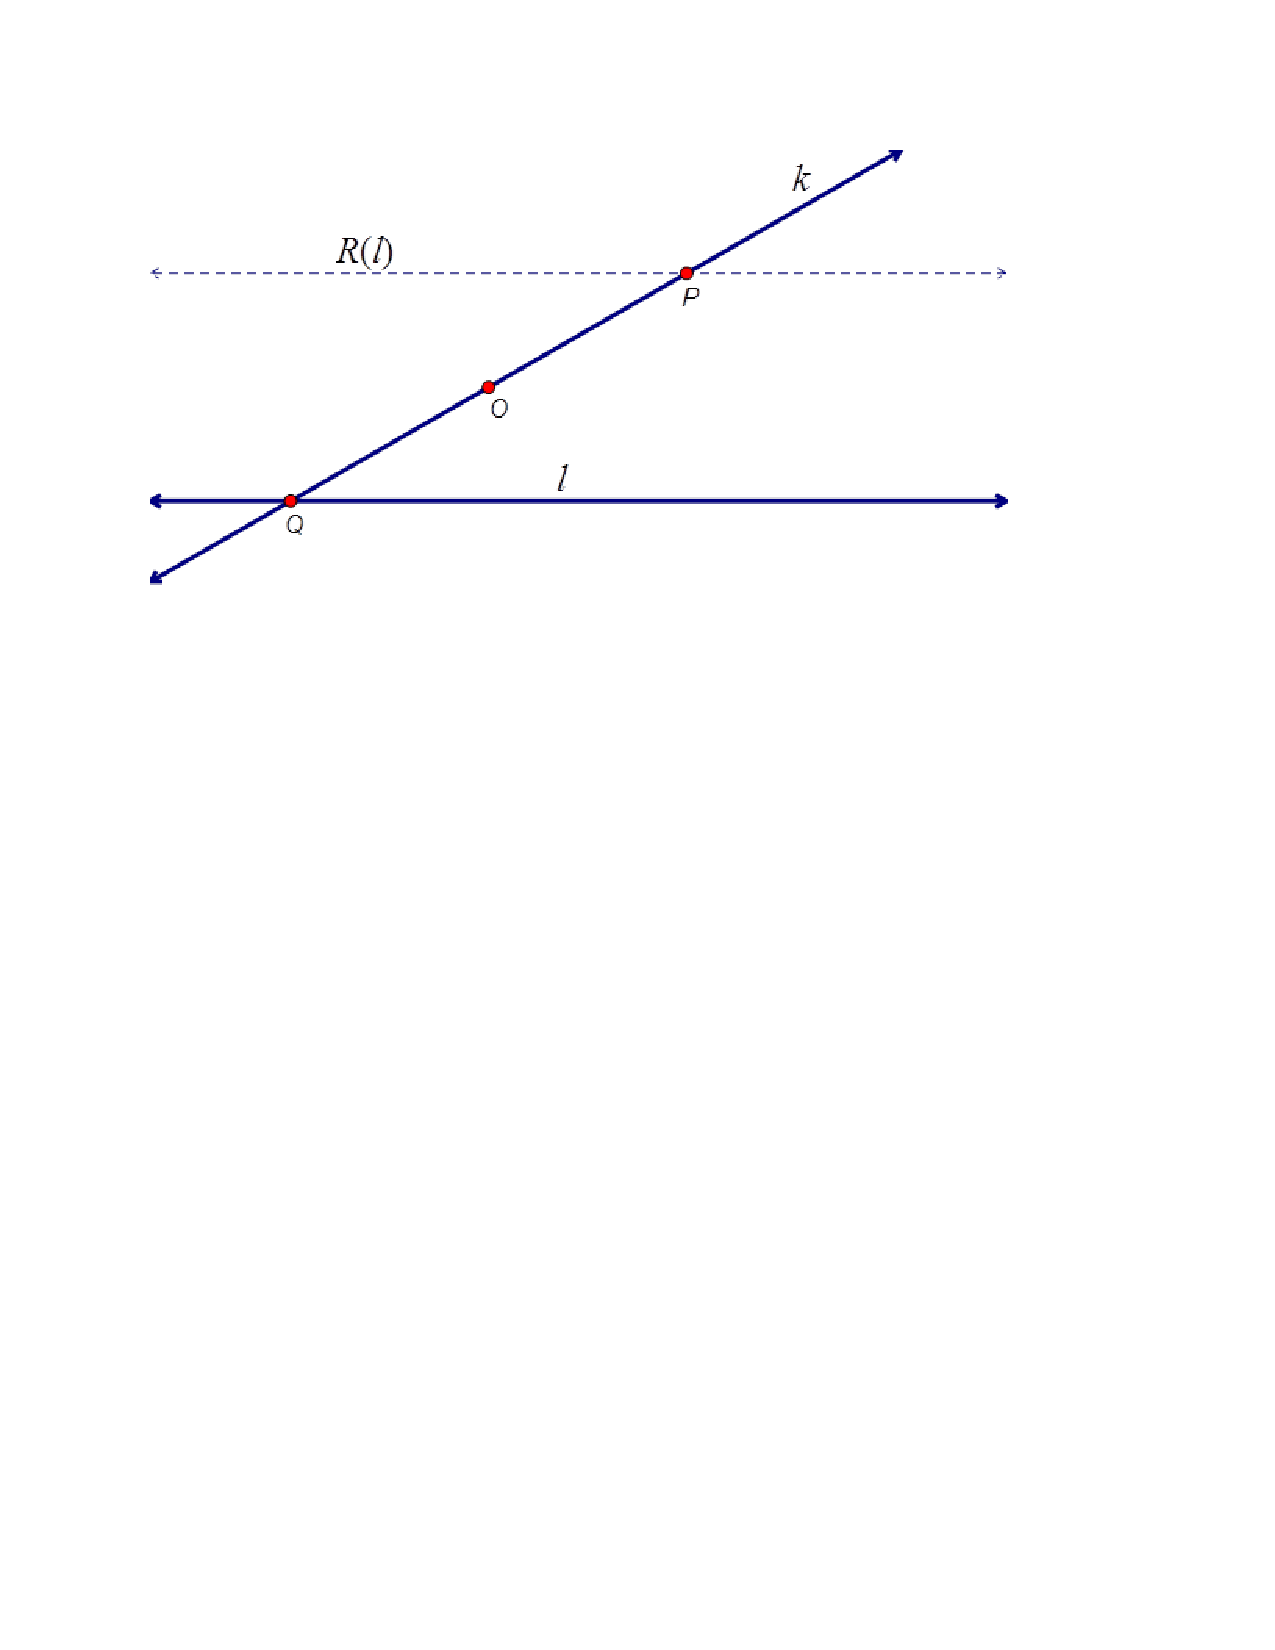
\includegraphics[scale=0.6]{../graphics/lineRotation.pdf}
\]

Because $P$ is on $R(l)$, there is a point $Q$ on $l$ such that $P = R(Q)$.  The rotated image of the ray $OQ$ is the ray $OP$, and because $\angle QOP$ is $180^\circ$, it follows that $Q$, $O$, and $P$ are collinear.  Call that line $k$.  We know line $k$ is distinct from $l$ because $O$ is on $k$ but not on $l$.  Now, if $P$ were on $l$, then points $P$ and $Q$ would be on two distinct lines, $k$ and $l$, contradicting A1 (i.e., on two points there is a unique line).  The theorem is proved.  
\end{proof}

% Previous proof (indirect) 
%
%\begin{proof}
%Suppose $R(l)$ is not parallel to $l$.  Then $R(l)$ and $l$ have a point $Q$ in common.  Because $Q$ is on $R(l)$, there is a point $P$ on $l$, 
%so that $R(P) = Q$. Because $R$ is a $180^\circ$ rotation around $O$, the three points $P$, $Q$, and $O$ lie in a line $m$. But
%$Q$ is by assumption also a point in $l$, so $l$ and $m$  have two distinct points in common: $P$ and $Q$. 
%But $l$ and $R(l)$ are distinct because $O$ is on $m$ but not on $l$. We have a contradiction, and thus $R(l)$ must be parallel to $l$.  
%\end{proof}
%
%Lemma 1 (page 81) and Theorem 1 is proved.
%
%Corollary. Given a line L and point P not on L, there is a line parallel to L and
%passing through P.
%
%Pick Q on L.  Let O be the midpoint of PQ, and use Theorem 1.  
%
%Theorem 2. Two lines perpendicular to the same line are either identical or parallel


\begin{problems}
\begin{enumerate}
\item Use adjacent angles to prove that vertical angles are equal.    
\item Now use rotations to prove that vertical angles are equal.

\item Prove that alternate interior angles and corresponding angles of a transversal with respect to a pair of parallel lines are equal.
\item Prove that the sum of the interior angles of a triangle is $180^\circ$.
\item Prove: If a pair of alternate interior angles or a pair of corresponding angles of a transversal with respect to two lines are equal, then the lines are parallel.
\end{enumerate}
\end{problems}


\section{Dilations, Scaling, and Similarity}
In a previous section, we saw how transformations can be used as a foundation for describing congruence and explaining the triangle congruence criteria.  In this section, we show how transformations can be used to describe similarity.  Because the basic rigid motions all preserve distances, we need a new kind of transformation:  a dilation. 

\begin{definition}
Given a point $O$ and a positive number $r$, a \emph{dilation} about $O$ by scale factor $r$, is a mapping that takes a point $P$ to a point $P'$ so that $OP' = r\cdot OP$.  
\end{definition}

With this definition, rubber bands are natural tools for exploring dilations.  
Through explorations with rubber bands and with geometry software, we observe that a dilation has the following properties:\standardhs{G-SRT.1}%\standardhs{G-SRT.1a}\standardhs{G-SRT.1b}  

\begin{enumerate}[(i)]\parskip0pt\parsep0pt
\item It maps lines to lines, rays to rays, and segments to segments.
\item It changes distance by a factor of $r$, where $r$ is the scale factor of the dilation.
\item It maps every line passing through the center of dilation to itself, and it maps every line not passing through the center of the dilation to a parallel line.  
\item It preserves angle measure.
\end{enumerate}

We could assume these properties, just as we have assumed the properties of the basic rigid motions.  Instead, we use our assumptions about area to prove some of these properties.  These are the Side-Splitter Theorems.

Now we are ready to define similarity.\standard{8.G.4}  

\begin{definition}
A geometric figure is \emph{similar} to another if the second can be obtained from the first by a sequence of rotations, reflections, translations, and dilations.  
\end{definition}


%If the objects are similar, try to find a single dilation that demonstrates the similarity.   If you cannot find such a dilation, explain how you know you cannot.  


\subsection{Theorems for Similar Triangles}

We need to show that this general definition of similarity fits with our previous ideas about similar triangles.  Here is one way of thinking about similar triangles:  

\[
\tri ABC \sim \tri A'B'C' \qquad\Leftrightarrow \qquad\begin{array}{l}
\angle A \simeq \angle A'\\
\angle B \simeq \angle B' \\
\angle C \simeq \angle C'
\end{array}
\]

\begin{question} 
What does this mean?  
\end{question}
\QM

Here is another way of thinking about similar triangles:  
\[
\tri ABC \sim \tri A'B'C' \qquad\Leftrightarrow \qquad
\begin{array}{l}
AB = k\cdot A'B'\\
BC = k\cdot B'C' \\
CA = k\cdot C'A'
\end{array}
\]

\begin{question} 
What does this mean?  
\end{question}
\QM


Using merely the formula for the area of a triangle, we (meaning you)
will explain why the following important theorem is true. Throughout this 
discussion we will use the convention that when we
write $AB$ we mean the \textit{length} of the segment $AB$.


\begin{theorem}[Parallel-Side] 
\index{Parallel-Side Theorem}\index{Theorem!Parallel-Side}
Given:
\[
\includegraphics{../graphics/split1.pdf}
\]
If side $BC$ is parallel to side $DE$, then
\[
\frac{AB}{AD} = \frac{AC}{AE}.
\] 
\end{theorem}

\begin{question}
Can you tell me in English what this theorem says?  How does it relate to the definition of similarity in terms of rigid motions and dilations?  
\end{question}
\QM

Now we (meaning you) are going to explore a bit. See if answering
these questions sheds light on this.

\begin{question} 
If $h$ is the height of $\tri ABC$, find formulas for the areas of
$\tri ABC$ and $\tri ADC$.
\[
\includegraphics{../graphics/split2.pdf} \qquad \includegraphics{../graphics/split3.pdf}
\]
\end{question}
\QM

\begin{question} 
If $g$ is the height of $\tri ACB$, find formulas for the areas of
$\tri ACB$ and $\tri AEB$.
\[
\includegraphics{../graphics/split4.pdf} \qquad \includegraphics{../graphics/split5.pdf}
\]
\end{question}
\QM


\begin{question} Explain why 
\[
\mathrm{Area}(\tri ABC) = \mathrm{Area}(\tri ACB).
\]
\end{question}
\QM

\begin{question} Explain why 
\[
\mathrm{Area}(\tri CBE) = \mathrm{Area}(\tri CBD).
\]
Big hint: Use the fact that you have two parallel sides! Draw a
picture to help clarify your explanation.
\end{question}
\QM

\begin{question} Explain why 
\[
\mathrm{Area}(\tri ADC)= \mathrm{Area}(\tri AEB).
\]
\end{question}
\QM

\begin{question}
Explain why
\[
\frac{\mathrm{Area}(\tri ABC)}{\mathrm{Area}(\tri ADC)} = \frac{ \mathrm{Area}(\tri ACB)}{\mathrm{Area}(\tri AEB)}
\]
\end{question}
\QM

\begin{question} Compute and simplify both of the following expressions:
\[
\frac{\mathrm{Area}(\tri ABC)}{\mathrm{Area}(\tri ADC)} \qquad\text{and}\qquad\frac{ \mathrm{Area}(\tri ACB)}{\mathrm{Area}(\tri AEB)}
\]
\end{question}
\QM


\begin{question} How can you conclude that: 
\[
\frac{AB}{AD} = \frac{AC}{AE}
\]
\end{question}
\QM

\begin{question} 
Why is it important that line $DE$ is parallel to line $CB$?
\end{question}
\QM


\begin{question} 
Can you sketch out (in words) how the questions above prove the Parallel-Side
Theorem?
\end{question}
\QM

Now comes the moment of truth. 
\begin{question}
Can you use the Parallel-Side Theorem to explain why if you know that
if you have two triangles, $\tri ABC$ and $\tri A'B'C'$ with:
\begin{align*}
\angle A &\simeq \angle A'\\
\angle B &\simeq \angle B' \\
\angle C &\simeq \angle C'
\end{align*}
then we must have that
\begin{align*}
AB &= k\cdot A'B'\\
BC &= k\cdot B'C'\\
CA &= k\cdot C'A'
\end{align*}
\end{question}
\marginnote{These notes do not describe why side $CA$ is also scaled by $k$.  You address that question in the Side-Splitter
Theorem activity.}
\QM


\subsubsection{The Converse}

The converse of the Parallel-Side Theorem states:

\begin{theorem}[Split-Side]\index{Split-Side Theorem}\index{Theorem!Split-Side} 
Given:
\[
\includegraphics{../graphics/split1.pdf}
\]
If side $BC$ intersects (splits) the sides of $\tri ADE$ so that
\[
\frac{AB}{AD} = \frac{AC}{AE},
\] 
then side $BC$ is parallel to side $DE$.
\end{theorem}

%\begin{question} 
%How could you investigate this theorem using any of the construction
%techniques above?
%\end{question}
%\QM

Now we (meaning you) will answer questions in the hope that they will
help us see why the above theorem is true.

\begin{question}
Suppose that you \textbf{doubt} that side $BC$ is parallel to side $DE$. Explain
how to place a point $C'$ on side $AE$ so that side $BC'$ is
parallel to line $DE$. Be sure to sketch the situation(s).
\end{question}
\QM

\begin{question} 
You now have a triangle $\tri ADE$ whose sides are split by a line
$BC'$ such that the line $BC'$ is parallel to line $DE$. What does the
Parallel-Side Theorem have to say about this?
\end{question}
\QM

\begin{question} What can you conclude about points $C$ and $C'$?
\end{question}
\QM


\begin{question} 
What does this tell you about the Split-Side Theorem?
\end{question}
\QM




Let's see if you can put this all together:
\begin{question}
Can you use the Split-Side Theorem to explain why you know that
if you have two triangles, $\tri ABC$ and $\tri A'B'C'$ with:
\begin{align*}
AB &= k\cdot A'B'\\
BC &= k\cdot B'C'\\
CA &= k\cdot C'A'
\end{align*}
then we must have that
\begin{align*}
\angle A &\simeq \angle A'\\
\angle B &\simeq \angle B' \\
\angle C &\simeq \angle C'
\end{align*}
\end{question}
\QM

Putting all of our work above together, we may now say the following:





\begin{theorem}\index{similar triangles} 
Two triangles $\tri ABC$ and $\tri A'B'C'$ are 
\textbf{similar} if either equilvalent condition holds:
\[
\begin{array}{l}
\angle A \simeq \angle A'\\
\angle B \simeq \angle B' \\
\angle C \simeq \angle C'
\end{array}
\qquad\text{or}\qquad
\begin{array}{l}
AB = k\cdot A'B'\\
BC = k\cdot B'C' \\
CA = k\cdot C'A'
\end{array}
\]
\end{theorem}

\begin{question}
How does this theorem connect back to the definition of similarity in terms of rigid motions and dilations? 
\end{question}
\QM


\fixnote{Possibly add section on SAS Similarity}

%
%   The following theorem 
%
%\subsubsection{SAS-Similarity Theorem}
%
%
%\begin{theorem}[SAS-Similarity Theorem]
%\index{Theorem!SAS Similarity}\index{SAS-Similarity Theorem} Knowing
%the ratio of the lengths of two sides and the measure of the angle
%between them, determines a triangle up to similarity. In pictures, we have something like:
%\[
%\includegraphics{../graphics/split1.pdf}
%\]
%\[
%\frac{AB}{AC} = \frac{AD}{AE} \qquad\Rightarrow\qquad \tri ABC \simeq \tri ADE.
%\]
%\end{theorem}
%
%\begin{question} What does this mean, ``up to similarity?''
%\end{question}
%\QM

%Let's see if we (meaning you) can get to the bottom of why this
%theorem is true. This time, you're going to produce the
%illustrations. Use folding and tracing why not!
%
%\begin{question}
%Fold any triangle. Now fold another triangle sharing one of the angles
%so that the ratio of the lengths of the sides are the same in both
%triangles. The sides touching the angle should share folds. You should
%see some parallel lines. Which theorem above says that this should
%happen?
%\end{question}
%\QM
%
%\begin{question} 
%What do we know about parallel lines crossing another line?
%\end{question}
%\QM
%
%\begin{question} 
%Can you sketch out (in words) how the questions above prove the SAS-Similarity
%Theorem?
%\end{question}
%\QM


\subsection{A New Meaning of Multiplication}
School mathematics makes sense when concepts have \emph{meaning}.  

\begin{question} 
What can multiplication mean?  Can you give multiplication meaning involving groups of groups or
something of the sort?
\end{question}
\QM

\begin{question} 
Can you give multiplication meaning involving areas or something of the sort?
\end{question}
\QM

\begin{question} 
Can you somehow give meaning to multiplication using similarity?  Use ``scale factor'' or ``scaling'' in your explanation.
\end{question}
\QM

\newpage 

\subsection{Problem Solving with Similarity} 


\fixnote{Following are rough notes.} 
We now have several ways of thinking more deeply about the naive ``same shape'' notion of similarity, imagined as zooming in and out.  In this section, we defined similarity in terms of basic rigid motions and dilations, and we used calculations involving area to show that these ideas are consistent with triangle similarity described as ``same angles''  or described as ``proportional sides.''

Again, the advantage of defining simlarity in terms of basic rigid motion and dilations, is that the approach 
applies not just to polygons but to figures of any shape.  And the key is identifying the scale factor.  

% Multiplication is not necessarily scaling--unless it is dilation
% Direct proportion versus not.  
% (e.g., baby from PowerPoint, types of televisions)

Here are some key ideas that arise in the activities and homework problems: 
\begin{enumerate}
\item Many real-world problems can be solved using similar triangles or other similar figures.  For example, you can use shadows to 
compute the height of a flagpole.  Maps, scale drawings, and scale models all involve similarity.  

\item A crticial issue is being able to distinguish situations in which figures are similar from those in which they are not.  

\item When using proportional relationships between corresponding parts of similar figures, it helps distinguish ``within figure'' ratios from ``across figure'' ratios, the latter being a scale factor.\standardhs{G-SRT.2}  When figures overlap, one challenge is being consistent about part-part versus part-whole ratios.

\item You may use the definition of similarity to show that any two circles are similar.\standardhs{G-C.1}  You can also see the more surprising result that any two parabolas are similar.  

\item Similarity turns out to be very useful in right triangles.  First, the altitude to the hypotenuse creates two triangles similar to the first.  Second, among right triangles, similarity requires specifying only one more angle, which leads to right triangle trigonometry.  
\end{enumerate}


\begin{problems}
\begin{enumerate}
\item Compare and contrast the ideas of \textit{equal triangles},
  \textit{congruent triangles}, and \textit{similar triangles}.
\item Explain why all equilateral triangles are similar to each other.
\item Explain why all isosceles right triangles are similar to each other. 
\item Explain why when given a right triangle, the altitude of the
  right angle divides the triangle into two smaller triangles each
  similar to the original right triangle.
\item The following sets contain lengths of sides of similar
  triangles. Solve for all unknowns---give all solutions. In each case
  explain your reasoning.
\begin{enumerate}
\item $\{3,4,5\}$, $\{6,8,x\}$
\item $\{3,3,5\}$, $\{9,9,x\}$
\item $\{5,5,x\}$, $\{10,4,y\}$
\item $\{5,5,x\}$, $\{10,8,y\}$
\item $\{3,4,x\}$, $\{4,5,y\}$ 
\end{enumerate}
\item A \textit{Pythagorean Triple}\index{Pythagorean Triple} is a set
  of three positive integers $\{a,b,c\}$ such that $a^2 + b^2 =
  c^2$. Write down an infinite list of Pythagorean Triples. Explain
  your reasoning and justify all claims.
\item Here is a right triangle, note it is \textbf{not} drawn to
  scale:
\[
\includegraphics{../graphics/origamiSimQ.pdf}
\]
Solve for all unknowns in the following cases.
\begin{enumerate}
\item $a = 3$, $b = ?$, $c = ?$, $d = 12$, $e = 5$, $f = ?$
\item $a = ?$, $b = 3$, $c = ?$, $d =8$, $e = 13$, $f = ?$
\item $a = 7$, $b = 4$, $c = ?$, $d =?$, $e = 11$, $f = ?$
\item $a = 5$, $b = 2$, $c = ?$, $d =6$, $e = ?$, $f = ?$
\end{enumerate}
In each case explain your reasoning.

\item Suppose you have two similar triangles. What can you say about
  the area of one in terms of the area of the other? Be specific and
  explain your reasoning.

\item During a solar eclipse we see that the apparent diameter of the
  Sun and Moon are nearly equal. If the Moon is around $240000$ miles
  from Earth, the Moon's diameter is about $2000$ miles, and the Sun's
  diameter is about $865000$ miles how far is the Sun from the Earth?
\begin{enumerate}
\item Draw a relevant (and helpful) picture showing the important
  points of this problem.
\item Solve this problem, be sure to explain your reasoning.
\end{enumerate}


\item When jets fly above $8000$ meters in the air they form a vapor
  trail. Cruising altitude for a commercial airliner is around $10000$
  meters. One day I reached my arm into the sky and measured the
  length of the vapor trail with my hand---my hand could just span the
  entire trail. If my hand spans $9$ inches and my arm extends $25$
  inches from my eye, how long is the vapor trail? Explain your
  reasoning.
\begin{enumerate}
\item Draw a relevant (and helpful) picture showing the important
  points of this problem.
\item Solve this problem, be sure to explain your reasoning.
\end{enumerate}

\item David proudly owns a 42 inch (measured diagonally) flat screen
  TV. Michael proudly owns a 13 inch (measured diagonally) flat screen
  TV. Dave sits comfortably with his dog Fritz at a distance of 10
  feet. How far must Michael stand from his TV to have the ``same''
  viewing experience?  Explain your reasoning.
\begin{enumerate}
\item Draw a relevant (and helpful) picture showing the important
  points of this problem.
\item Solve this problem, be sure to explain your reasoning.
\end{enumerate}

\item You love IMAX movies. While the typical IMAX screen is 72 feet
  by 53 feet, your TV is only a 32 inch screen---it has a 32 inch
  diagonal. How close do you have to sit to your screen to simulate
  the IMAX format? Explain your reasoning.
\begin{enumerate}
\item Draw a relevant (and helpful) picture showing the important
  points of this problem.
\item Solve this problem, be sure to explain your reasoning.
\end{enumerate}

\item David proudly owns a 42 inch (measured diagonally) flat screen
  TV. Michael proudly owns a 13 inch (measured diagonally) flat screen
  TV. Michael stands and watches his TV at a distance of 2 feet. Dave
  sits comfortably with his dog Fritz at a distance of 10 feet. Whose
  TV appears bigger to the respective viewer? Explain your reasoning.
\begin{enumerate}
\item Draw a relevant (and helpful) picture showing the important
  points of this problem.
\item Solve this problem, be sure to explain your reasoning.
\end{enumerate}

\item Here is a personal problem: Suppose you are out somewhere and
  you see that when you stretch out your arm, the width of your thumb
  is the same apparent size as a distant object. How far away is the
  object if you know the object is:
\begin{enumerate}
\item 6' long (as tall as a person).
\item 16' long (as long as a car).
\item 40' long (as long as a school bus).
\item 220' long (as long as a large passenger airplane).
\item 340' long (as long as an aircraft carrier).
\end{enumerate}
Explain your reasoning.

\item I was walking down Woody Hayes Drive, standing in front of
  St.\ John Arena when a car pulled up and the driver asked, ``Where
  is Ohio Stadium?'' At this point I was a bit perplexed, but
  nevertheless I answered, ``Do you see the enormous concrete building
  on the other side of the street that looks like the Roman Colosseum?
  That's it.''
 
The person in the car then asked, ``Where are the Twin-Towers then?''
Looking up, I realized that the towers were in fact just covered by
top of Ohio Stadium. I told the driver to just drive around the
stadium until they found two enormous identical towers---that would be
them. They thanked me and I suppose they met their destiny.

I am about 2 meters tall, I was standing about 100 meters from the
Ohio Stadium and Ohio Stadium is about 40 meters tall. If the Towers
are around 500 meters from the rotunda (the front entrance of the
stadium), how tall could they be and still be obscured by the stadium?
Explain your reasoning---for the record, the towers are about 80
meters tall.


\item Explain how to use the notion of similar triangles to multiply
  numbers with your answer expressed as a segment of the appropriate
  length.

\item Explain how to use the notion of similar triangles to divide
  numbers with your answer expressed as a segment of the appropriate
  length.


\item Consider the following combinations of S's and A's. Which of
  them produce a \textit{Congruence Theorem}? Which of them produce a
  \textit{Similarity Theorem}? Explain your reasoning.
\[
\text{SSS},\quad \text{SSA},\quad \text{SAS},\quad 
\text{SAA},\quad \text{ASA},\quad \text{AAA} 
\]


\item Explain how the following picture ``proves'' the Pythagorean Theorem.
\[
\includegraphics[scale=0.8]{../graphics/pbpdilation.pdf}
\]


%\item \label{P:CP} Given a circle centered at point $O$, we'll call
%  two points $P$ and $P'$ a \textit{connected pair} if:
%\begin{enumerate}
%\item $O$, $P$, and $P'$ all lie on a line.
%\item $OP = \dfrac{1}{OP'}$.
%\end{enumerate}
%For example, if the radius of the circle was $12$ and $P$ was $6$
%units from $O$, then $P'$ would be $18$ units from $O$. Give some
%other examples of connected pairs.
%\item If $P$ and $P'$ are a connected pair (see Problem~\ref{P:CP})
%  and $P$ is on the circle, what can you say about $P'$? Explain your
%  reasoning.
%\item Consider the following diagram where $P$ and $P'$ are connected
%  pairs (see Problem~\ref{P:CP}):
%\[
%\includegraphics{../graphics/origamiConnected.pdf}
%\]
%What is the distance $P'Q'$? Hint: Try to use the SAS-Similarity
%Theorem, to do this you'll have to find some sides with common ratios!

\end{enumerate}
\end{problems}


\section{Length, Area, and Volume Under Scaling}

\fixnote{This section needs elaboration.}

When two objects are similar, then lengths are related by a scale factor.  What does this mean for other measurements, such as perimeters, areas, volumes, weights, etc.  

Here are some ideas to think about:  

\begin{itemize}\itemsep-2pt
\item General considerations of measurement and dimension.  
\item Making scale drawings and on using scale drawings to solve problems about length and area
\item Reason about length, area, and volume in similarity situations.  Rep-tiles.    
\item Use shearing and Cavalieri's principle to reason about area and volume.  
\item Using a grid (and scaling the grid) to reason about areas of general shapes under scaling.  
\item Volume as area of base times height:  Imagine layers of cubic units covering the base.
\item Volume of pyramid:  Three pyramids make a cube.  
\item Volume of cylinder, cone, and sphere.
\item If you know the area of a rectangle, what can you say about its perimeter?  What about more general figures?  
\item If you know the perimeter of a rectangle, what can you say about its area?  What about more general figures? 
\item Fractals are ``self-similar'' figures.  
\end{itemize}

 


